\documentclass[12pt,oneside,titlepage,openright,a4paper]{book}
\usepackage[utf8x]{inputenc}
\usepackage[comma,sort&compress,super,sort]{natbib}
\usepackage[version=3]{mhchem} % Formula subscripts using \ce{}
\usepackage{pdflscape}
\usepackage{ucs}
%\usepackage{uarial}
\usepackage[spanish,english]{babel}
\usepackage{latexsym}
\usepackage{amssymb,amsmath,amsthm,amsfonts}
\usepackage{fancyhdr}
\usepackage{fancybox}    
\usepackage{t1enc}
\usepackage{array}
\usepackage[pdftex]{graphicx}
\usepackage[below]{placeins}
\usepackage{float}
\usepackage{caption}
\usepackage{rotating,colortbl,longtable,tabulary,booktabs}
\usepackage{tocbibind}
\usepackage{wrapfig,subfigure}
\usepackage{tikz,pgfkeys,tkz-base}
\usepackage{comment} % enables the use of multi-line comments (\ifx \fi)
\usepackage{fullpage} % changes the margin
\usepackage{multirow, array}
\usepackage[left=3cm,right=2.5cm,top=2cm,bottom=2cm]{geometry}
\usepackage{appendix}
\usepackage{lmodern}
\usepackage{booktabs}
\usepackage{lscape}
\usepackage{pdflscape}
\usepackage{rotating}
\usepackage{url}
% \newcounter{subsubsubsection} [subsubsection]
\setcounter{secnumdepth}{3}
\usetikzlibrary{arrows,decorations.pathmorphing,backgrounds,positioning,fit,trees,calc,through,plotmarks}
%\bibpunct{}{,}{} 
\setlength{\parindent}{0.5cm}
\setlength{\parskip}{0.2cm}
\linespread{1.5}
\usepackage{eso-pic}
\newcommand\BackgroundPic{
\put(0,0){
\parbox[b][\paperheight]{\paperwidth}{%
\vfill
\centering

\includegraphics[width=0.75\paperwidth,height=\paperheight,keepaspectratio]{figuras/ib.png}%
\vfill
}}}
%--------------------------------------------------------------------------------------------------------------------------------------------------------------------
\begin{document}
\AddToShipoutPicture{\BackgroundPic}
\renewcommand{\tablename}{Tabla}
\renewcommand{\listtablename}{Índice de Tablas}
\renewcommand{\contentsname}{Contenido}
\renewcommand{\listfigurename}{Índice de Figuras}
\renewcommand{\chaptername}{Capítulo}
\begin{titlepage}
\begin{center}
\textbf{\begin{LARGE}Universidad Católica de Santa María \end{LARGE}}\\
\begin{Large}Facultad de Ciencias Farmacéuticas, Bioquímicas y Biotecnológicas\end{Large}\\
\begin{large}Escuela profesional de Ingeniería Biotecnológica\end{large}\\\vspace{2.0cm}

\includegraphics[scale=0.3]{figuras/logo.png}\\\vspace{2.0cm}
\textbf{\begin{LARGE} Titulo
\end{LARGE}}\\\vspace{2.0cm}
\end{center}
\begin{flushright}
\begin{minipage}{7cm}
Tesis presentada por el Bachiller:\\ \textbf{Apellidos y Nombres}\\ 
Para Optar el Titulo Profesional de:\\  \textbf {Ingeniero Biotecnólogo} \\
Asesor:\\ Nombre del Asesor
\end{minipage}
\end{flushright}
\vspace{0.5cm}
\begin{center}
\begin{Large}\textbf{Arequipa -- Perú\\2023}\end{Large}
\end{center}
\end{titlepage}
%--------------------------------------------------------------------------------------------------------------------------------------------------------------------
\pagenumbering{arabic}\tableofcontents 
%--------------------------------------------------------------------------------------------------------------------------------------------------------------------
\chapter{Introducción}


\chapter{Planteamiento de la Investigación}
\renewcommand{\figurename}{Figura}
La Diabetes se encuentra entre las diez enfermedades con alta mortalidad en adultos, presentando una prevalencia del 9,3\% en el año 2019 y según predicciones se puede esperar un aumento del 0,9\% para el año 2030. %Rachin%
Esta alarma no es indiferente a la búsqueda de soluciones alternativas para tratar mencionada enfermedad, existen diversos métodos y tratamientos que se han expuesto a la sociedad como son medicamentos asociados a reducir la glucosa en la sangre como los son la metformina que es uno de más usados actualmente.%Buscar idea%
Las investigaciones nos indican que existen otros blancos disponibles como lo es el tratamiento de la DMT2 aumentando la prevalencia de la activación de la via de señalización dependiente de GLP1, evitando su inhibición por la enzima Dipeptidil peptidaza 4 (DPP4) mencionada proteína puede inhibirse por diversos fármacos del grupo de las gliptinas, como lo es la Vildagliptina entre otras. %Buscaridea%

Se ha querido encontrar diversos metabolitos que puedan evitar la interacción farmacéutica o solo reducirla para poder ser reemplazada por algún metabolito proveniente de agentes naturales como lo son las plantas. %buscar idea%
En esta investigación nos centraremos en el potencial de diversos metabolitos encontrados en el aloe vera para poder ser comparados y encontrar diferencias significativas entre el uso de los agentes farmacológicos y los agentes naturales. viendo las diferencias podremos afirmar si los agentes derivados del aloe vera podrían ser similares, o mejores que los agentes farmacológicos. %buscar idea% 

\section{Problemática de la investigación}

Según lo encontrado por Rachi et al podemos afirmar que la prevalencia de Diabetes irá en aumento hasta llegar a un nivel de aumento del 0,9-1\% de prevalencia en aproximadamente 5 años, es por ello que se requiere de nuevas tecnologías que puedan ayudar al tratamiento o control de mencionada patología.
Dentro de la problemática principal como lo es el aumento de la prevalencia de los casos de diabetes a nivel global, esto trae consigo problemas asociados como lo son las neuropatías, daño renal, retinopatías entre otras.%Publications%
Por otro lado se ha observado que la Metformina ha empezado a presentar algunos efectos secundarios en gente adulta como lo son malestares gástricos e intestinales los cuales han forzado a los tratamientos ayudarse del grupo de los fármacos como las gliptinas para poder ayudar a estos cambios siendo la solución la inhibición de la proteína DPP4.

Finalmente el consumo de fármacos seguirá en crecimiento durante este aumento de la prevalencia de Diabetes es por ello que es mejor optar por otras opciones aparte de los fármacos y tratamientos convencionales enfocándonos en la naturaleza, es por ello que haciendo un análisis de posibles inhibidores postulamos al aloe vera como uno de los posibles portadores de metabolitos secundarios que puedan contener compuestos que interaccionen a nivel del intestino y estómago con fundamento a los antecedentes que presenta mencionada planta frente a la diabetes.

\section{Pregunta de investigación}
Dentro del análisis de datos obtenidos de los antecedentes del aloe vera con la diabetes ¿Es posible mencionar que los metabolitos secundarios encontrados en el aloe vera presenten mayor capacidad inhibitoria que los  fármacos convencionales que interactúan con la proteína DPP4 para el control de la Diabetes Mellitus tipo 2 (DMT2)?

\section{Justificación}
%social 
En el ámbito social, presentamos multiples falencias como es la evolución lenta de implementación de nuevas técnicas de organización nacional sanitaria, esto se demuestra en las estadísticas encontradas sobre la prevalencia de diabetes en el Perú cuyo estado predice un aumento de prevalencia de la enfermedad en estos años, es por ello que una de las soluciones es emplear nuevas tecnologías para que esta y muchas de las nuevas tecnologías podría brindarnos alternativas para poder emplear metabolitos naturales de plantas nativas del Perú para así brindar un respaldo de prevención y control de la enfermedad frente a la poca distribución de fármacos o pacientes cuyo tratamiento diario con medicamentos sintéticos generando asi posibles resistencias en el organismo.  


%tecnológica
Se ha visto que diversos métodos aplicados para el tratamiento de la diabetes mellitus tipo 2, y debido a la prevalencia nacional encontrada que nos habla de 7\% de prevalencia en Perú. Tomamos en cuenta que, las nuevas tecnologías son la esperanza de evitar grandes gastos en el control de enfermedades y síntesis de fármacos, en este caso las tecnologías de predicción de interacciones y resultados pre-experimentales nos ayudan a dilucidar que diferentes metabolitos naturales podrían tener un efecto igual o superior a los fármacos comúnmente comercializados para el fin de la inhibición de la enzima DPP4. 
Por otra parte los resultados obtenidos nos abrirán paso a nuevas aplicaciones de plantas importantes empleadas actualmente como medicina alternativa al consumo excesivo de medicamentos sintéticos, finalmente al emplear de nuevas tecnologías computacionales en el tratamiento de la diabetes mellitus como lo es la bioinformática nos podría ayudar a encontrar respuesta no solo a nuevos metabolitos, sino también las barreras de aplicación de tratamientos a personas cuya genética rechaza tratamientos convencionales.%

%Resultados La prevalencia nacional estimada de diabetes fue del 7,0\% (IC del95\% 5,3\% a 8,7\%) y fue de 8,4\% (IC del 95\% 5,6\% a 11,3\%) en Lima metropolitana. 
%Ventajas de la biología computacional: Explicar las ventajas del enfoque computacional para estudiar la interacción enzima-inhibidor. Mencionar técnicas específicas que se utilizarán (ej: docking molecular, dinámica molecular, análisis de componentes principales) y cómo estas técnicas ayudarán a superar las limitaciones de los métodos experimentales. Detallar las bases de datos o software que se utilizarán.

%Hipótesis y objetivos: Formular una hipótesis específica y clara sobre la interacción y definir los objetivos de la tesis. Estos objetivos deben estar directamente relacionados con el hueco de conocimiento identificado. Los objetivos deben ser medibles y alcanzables en el marco de una tesis de pregrado.
%Originalidad (a nivel de pregrado): Aunque puede que no se trate de una investigación completamente novedosa a nivel mundial, se debe justificar la originalidad del trabajo a nivel de pregrado. Esto podría implicar:
 %   El análisis de una nueva variante de la enzima o inhibidor.
 %   La aplicación de una nueva metodología computacional a un sistema previamente estudiado.
  %  Un enfoque novedoso en el análisis de los datos obtenidos.
  %  Una combinación de diferentes técnicas computacionales para un análisis más completo.
%DOI
%https://doi.org/10.1016/j.compbiolchem.2024.108145
  %Base de datos
%https://www.ebi.ac.uk/chembl/explore/drug_mechanisms/STATE_ID:wFt0kVdHXqmQoTue0brSuQ%3D%3D

%ambieltal
En el Perú se encuentra una de las mayores base multidiversificadas de flora y fauna de Sudamérica. En esta ocasión se explica algunas de las ventajas de una especie de las múltiples variedades de flora que existe en el país, el aloe vera; demostrando la riqueza que podemos encontrar en la química extraída de forma natural en las plantas. Es por ello, que considero, que reportes que nos ayuden a generar conciencia de cuidar la diversificación de la flora son necesarios debido a las aplicaciones que podemos encontrar en ellas, sin necesidad del uso de gasto económico en recursos para síntesis de medicamentos y reduciendo considerablemente contaminantes de suelo y agua a partir de medicamentos que no son metalizados completa o parcialmente por nuestro organismo y que en muchas ocasiones llegan a ser desechados  sin tomar importancia del gran impacto que estos pueden tener frente a animales y plantas.

Es por ello que este proyecto tiene como uno de los objetivos el argumentar en la importancia del cuidado de la flora resaltando la importancia que estas plantas podrían tener y ayudando a reducir el consumo excesivo de medicamentos, optimizando los tratamientos convencionales y concientizar acerca del cuidado ala naturaleza.

\section{Alcance}
La presente investigación se desarrollará bajo un alcance descriptivo-correlacional, con el propósito de analizar comparativamente los metabolitos del aloe vera y los fármacos convencionales en relación con su poder inhibitorio de la proteína DPP4.
El componente descriptivo permitirá caracterizar detalladamente las propiedades moleculares de los metabolitos del aloe vera, documentando sus características estructurales y comportamiento bioquímico. Simultáneamente, el enfoque correlacional facilitará el establecimiento de relaciones sistemáticas entre los diferentes compuestos, permitiendo cuantificar y comparar su capacidad inhibitoria.
Se contempla un análisis exhaustivo que incluirá la identificación de metabolitos activos, la evaluación de su potencial farmacológico y la determinación de correlaciones estadísticamente significativas entre los diferentes compuestos estudiados. El objetivo central radica en comprender la potencial eficacia del aloe vera como alternativa terapéutica en la modulación de la enzima DPP4.

\section{Objetivos}

\subsection{General}
Evaluar el poder inhibitorio de los metabolitos del aloe vera frente a fármacos usados en terapias contra la Diabetes Mellitus tipo 2 (DMT2) sobre la proteína DPP4, determinando su potencial terapéutico y mecanismo de acción molecular.

\subsection{Específicos}

\begin{itemize}
 \item Identificar las características metabólicas encontradas en la hidrólisis de la proteína GLP1 por la enzima DPP4 en sus estados basales
 \item Analizar y generar una base de datos de metabolitos de alto interés clínico proveniente del Aloe Vera al igual que de fármacos de alta importancia en el tratamiento de la diabetes mellitus tipo 2 
 \item Cuantificar y comparar la capacidad inhibitoria de los metabolitos del aloe vera con fármacos convencionales utilizando softwares de biología computacional, determinando y evidenciando los mecanismos de interacción molecular.

\end{itemize}

\section{Hipótesis}
Ante todo lo mencionado y en objetivo a resolver la pregunta de investigación planteada, procedemos a construir la siguiente hipótesis:

Los metabolitos encontrados en el aloe vera presentarán propiedades inhibitorias superiores a los fármacos comerciales usados en la primera línea para el tratamiento de Diabetes Mellitus Tipo 2 (DMT2).  


\section{Variables e indicadores}

 \begin{table}[htbp]
 \caption{Cuadro de variables}\label{t1}
  \begin{tabular}{llcp{3.5cm}p{3.5cm}p{3.5cm}cp{3.5cm}}
  \hline
  \multicolumn{3}{c}{\textbf{Variables}}                       & \textbf{Variable}      & \textbf{Indicadores}                 & \textbf{Unidades} \\ \hline
  \multicolumn{3}{c}{\multirow{2}{*}{\textbf{Independientes}}} 
  & Ligandos & Propiedades fisicoquímicas & IC50,ADMET\\ \cline{4-6} 
  \multicolumn{3}{c}{}                                         &Proteínas  & Energía de interacción  & KJ/mol \\ \hline
  \multicolumn{3}{l}{\multirow{3}{*}{\textbf{Dependientes}}}   &Binding Energy   &Energía libre de Gibbs, Energía de interacción   & KJ/mol \\ \cline{4-6} 
  \multicolumn{3}{l}{}                                         &Proximidad Molecular   &Distancia entre átomos   &Angstroms \\ \cline{4-6} 
  \multicolumn{3}{l}{}                                         &Dinámica Molecular   &RMSD y RMSF   &nm/ns \\ \hline 
  \end{tabular}
\end{table}
%Independientes
%Metabolitos del aloe vera (identificados y seleccionados)
%Fármacos convencionales de referencia (identificados y seleccionados)
%Características fisicoquímicas de los ligandos

%Dependientes
%Valores de afinidad de unión (docking molecular)
%Porcentaje de inhibición calculado computacionalmente
%Cambios conformacionales de la proteína DPP4
\section{Tipo y Nivel de Investigación}
El tipo de investigación usada para este análisis es básica siendo una investigación fundamental ya que nos da a conocer una alternativa que no tiene aplicación inmediata pero si unos resultados validados en el campo cuántico químico y fisicoquímicas, generando resultados para el avance de tecnologías que podrían ayudar a la optimización de tratamientos contra la DMT2  



\chapter{Antecedentes}
\renewcommand{\figurename}{Figura}

\section{Estado del Arte}
Algunos libros como lo es publicado por "Exon Publications" donde se afirma que, la diabetes tipo 2 es una afección crónica caracterizada por la resistencia a la insulina y alteración de la secreción de insulina, lo que conduce a niveles elevados de glucosa en sangre. Esta publicaciòn nos brinda información sobre la Diabetes Tipo 2. Sus expplicaciones abarcan los tipos, factores de riesgo, epidemiología, causas, síntomas, fisiopatología, complicaciones, diagnóstico, tratamiento y pronóstico de Diabetes Tipo 2. 
Dentro de este libro nos muestran algunas de las afecciones añadidas a la diabetes como lo es la falla renal, neuropatías, retinoptologías y afecciones estomacales como ulceras, entre otros.\cite{Publications2024}

Dentro de el libro antes mencionado nos brindan las explicaciones del porque la diabetes es una afecciòn de alta preocupación entre la sociedad, y es necesario encontrar soluciones inmediatas. En el Perù tambien se encuentran muchos de estas...


El Aloe vera es una planta medicinal propia de la gran diversidad biológica. Algunos estudios previos demostraron el efecto antihiperglucémico de Aloe vera pero con resultados inconsistentes. 
Pero Indah et al en el artìculo "The effect of Aloe vera on fasting blood glucose levels in pre-diabetes and type 2 diabetes mellitus: A systematic review and meta-analysis" tuvo como objetivo asumir cuantitativamente el efecto de Aloe vera en el ayuno de glucosa en sangre en la pre-diabetes y diabetes mellitus tipo 2 mediante un metaanálisis.
Se usaron como buscadores principales para analizar ensayos clìnicos que pueden haber evaluado el aloe vera en el ayuno de glucosa en sangre publicado entre 2011 y 2021: PubMed, Scopus, Springer Link, Science Direct, Proquest, y Google Scholar. Se utilizó Aloe vera como la única intervención haciendo que el efecto agrupado de Aloe vera en la glucosa en sangre en ayunas se evaluó usando el modelo de efecto aleatorio, y el sesgo de publicación fue evaluado por las parcelas de Funnel y Fail Safe-N. En mencionado paper se tomaron los siguirntes resultados, mostrando que el Aloe vera redujo significativamente la glucosa en sangre en ayunas (-0,35 [IC 95\%, -1454, -0,616] mg/dL; p-0,001) en comparación con el control. 

El aloe vera puede tener un efecto más notable en los hombres, IMC no superior a 30 mg/kg2, diabetes mellitus tipo 2, administrado para una dosis superior a más de 8 semanas, dosis a 200 mg y administración de cápsulas. Sin embargo, se encontró una alta heterogeneidad en los estudios. Los que nos sugiere la productividad del Aloe Vera en el tratamiento de la diabetes mellitus tipo 2 $(DMT2)$.\cite{Budiastutik2022}







%En el artículo titulado "Phthalate-induced testosterone/androgen receptor pathway disorder on spermatogenesis and antagonism of lycopene" publicado en el año de 2022, se detalla que la vía de señalización de testosterona (T)/receptor de andrógenos (AR) está involucrada en el mantenimiento de la espermatogénesis y la fertilidad masculina. Los resultados obtenidos en la investigación demostraron que el ftalato de mono-2-etilhexilo (MEHP) causó daño mitocondrial y daño oxidativo, por lo que se determinó que esta sustancia química seria amenaza para el progreso de la espermatogénesis. Sin embargo, en la investigación también realizaron estudios antagonistas del licopeno frente a la alteración que produce los ftalatos en el trastorno de la vía del receptor de andrógenos/ testosterona, teniendo como resultados que este suplemento LYC es una agente antioxidante natural que inhibe los cambios producidos por los ftalatos frente la función espermatogénica de los testículos. En general, este estudio revelo un papel fundamental para la transducción de señales T/AR en la fertilidad masculina y proporciono información prometedora sobre el papel protector de LYC en los trastornos reproductivos masculinos inducidos por ftalatos.\cite{b12}



\chapter{Marco Teórico}

 \section {Título de la sección}
 
 
\subsection{Título de la subsección}



 
\chapter{Planteamiento Metodológico}

Para la metodología se optó por el campo computacional usando softwares especializados en lo que es interacciones y dinámicas moleculares

\section{Lugar en donde se desarrollará la investigación}
El lugar donde se desarrollará esta investigación es en Centro de Investigación en Ingeniería Molecular (CIIM) autorizado y supervisado por el Dr. Badhin Gómez Valdez   

\section{Ambientes por utilizar}
Se usaran los ambientes asociados al centro de investigación cuya estación de trabajo está preparada y optimizada para generar los resultados esperados dentro de la preparación, dinámica y análisis molecular. 

\section{Materiales}
Para esta investigación se han de requerir computadores óptimos para los cálculos cuánticos que se tienen que llevar a cabo:

\subsection{Hardware}
\begin{itemize}
    \item Procesador AMD Ryzen 9 
    \item Placa madre X570 gaming
    \item GPUs NVIDIA 3080 y NVIDIA 2080
    \item sistemas de ventilación optimizados
    \item Fuente de poder de Seasonic 80 Plus Gold
\end{itemize}

\subsection{Software}
\begin{itemize}
    \item Sistema operativo Linux 24.04
    \item Chimera X
    \item AlphaFold3 (Nativo)
    \item Autodock Vina (Nativo)
    \item Gromacs v.2024.3 
    \item Gaussian y derivados
\end{itemize}

\section{Métodos}

\subsection{Interacción proteica en estado basal de la enzima DPP4}
Para ello haremos uso de los softwares de predicción de modelos proteicos como lo es el modeller integrado en el software Chimera X al igual que AlphaFold3 que tienen la finalidad de predecir el estado de la proteína por comparación.

El primero objetivo a cumplir es la extracción de la proteína de una base de datos como lo es Protein Data Bank (PDB) luego de encontrar la enzima adecuada verificando la mejor valoración según bibliografía procedemos a realizar la construcción de la molécula si lo necesita, posterior a ello procedemos a la búsqueda de la proteína blanco como lo es el Péptido Parecido al Glucagón (GLP1) de la misma forma valoramos por búsqueda bibliográfica los estadios de la molécula y usamos softwares de modelado si esto lo requiere, Softwares como AlphaFold que mejora considerablemente al tenerlo integrado a la máquina donde se trabajará el modelado de las proteínas.

Después de haber realizado la limpieza de las proteínas y completado todos los residuos a utilizar si estos lo requieren. Generamos dinámicas moleculares usando GROMACS como software y OPLS como campo de fuerza a las proteínas por separado, esto con el fin de estabilizar ambas proteínas y encontrar su estado basal independiente gracias a los gráficos de dinámica.
Posterior a ello procederemos a la interacción proteica esto se realizará con un dockeo a nivel citoplasmático como es normalmente, en este caso mantenemos la GLP1 estable mientras que la enzima dse aproxima como ligando, normalmente mientras más veces repita el Autodock vina presenta mejor probabilidad estadística de brindar un resultado estable donde podemos afirmar el valor inhibitorio en estado basal de ambas moléculas cuando interaccionan en el estado de catálisis enzimática.

\subsection{Generación de la base de datos de ligandos}
Para este punto se requiere del análisis de bibliografía especializada en ligandos de interés como pueden ser ligandos encontrados en el Aloe Vera con aplicaciones antidiabéticas pero también los ligandos encontrados para otras funciones podrían ser resultados favorables es por ello que hacemos una búsqueda de aproximadamente 113 metabolitos gracias a diferentes bases de datos los cuales serán filtrados por bibliografía y por el estándar ADMET que nos ayudará a buscar los mejores resultados para tener valores altos de druagabilidad protética y así generar la inhibición de DPP4.

Finalmente usaremos la base de datos de estudios previos farmacológicos que nos agreguen la mayor cantidad de fármacos comerciales sintetizados con la finalidad de generar la inhibición de DPP4. Estos fármacos presentan a la familia de las gliptinas como una de las más importantes pero se agregarán muchos mas dependiendo del análisis bibliográfico y el filtro ADMET que nos ayudará a buscar estadísticamente los mejores resultados para la interacción como ligandos inhibidores de la actividad enzimática de la DPP4. 

\subsection{Análisis de resultados por dinámica molecular y análisis estadístico}
Dependiendo de los resultados generaremos un análisis de los mejores ligandos tanto de los ligandos sintéticos como de los de procedencia natural ya que la liste ha reducido considerablemente se pude realizar un ultimo dockeo con el fin de encontrar diferencias en las energías de interacción ya que de esta evaluación se generará un análisis estadístico para evidenciar los mejores ligandos con mejor potencial inhibitorio decidiendo finalmente si los metabolitos extraídos del aloe vera podrían superar la inhibición de los actuales fármacos usados para el tratamiento de la Diabetes Mellitus Tipo 2.
\newpage
\section{Flujograma de actividades}

\begin{figure}[h]
    \centering
    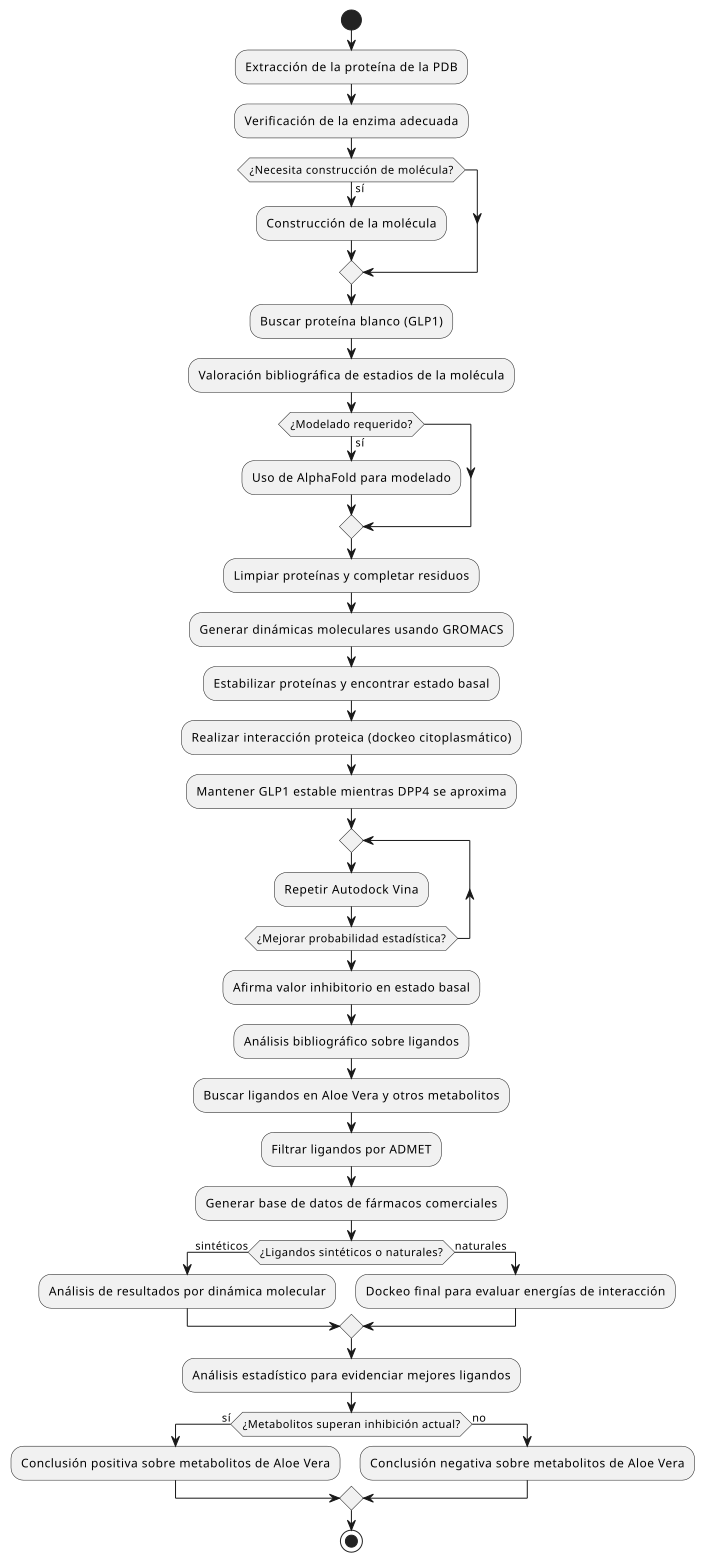
\includegraphics[scale=0.485]{figuras/Flujograma.png}
\end{figure}







\chapter{Cronograma y Presupuesto de la Investigación}

\newpage
\section{Cronograma} 
\begin{table}[!htb]
\begin{center}
\begin{tabular}{|p{7cm}|c|c|c|c|c|c|c|c|c|c|c|c|}\hline
\multirow{2}{*}{\textbf{Actividades}}    & \multicolumn {12}{c|}{\textbf{Meses}} \\\cline{2-13}
                                              & 1 & 2 & 3 & 4 & 5 & 6 & 7 & 8 & 9 & 10 & 11 & 12\\\hline
                                              &   &   &   &   &   &   &   &   &   &    &    &   \\\hline
                                              &   &   &   &   &   &   &   &   &   &    &    &   \\\hline    
                                              &   &   &   &   &   &   &   &   &   &    &    &   \\\hline
                                              &   &   &   &   &   &   &   &   &   &    &    &   \\\hline  
                                              &   &   &   &   &   &   &   &   &   &    &    &   \\\hline
                                              &   &   &   &   &   &   &   &   &   &    &    &   \\\hline  
                                              &   &   &   &   &   &   &   &   &   &    &    &   \\\hline
                                              &   &   &   &   &   &   &   &   &   &    &    &   \\\hline  
                                              &   &   &   &   &   &   &   &   &   &    &    &   \\\hline
                                              &   &   &   &   &   &   &   &   &   &    &    &   \\\hline  
                                              &   &   &   &   &   &   &   &   &   &    &    &   \\\hline
                                              &   &   &   &   &   &   &   &   &   &    &    &   \\\hline                                                
\end{tabular} 
\end{center}
\end{table}


\newpage
\section{Presupuesto}

Financiado por el fondo 
 
%\include{referencias}
%--------------------------------------------------------------- ---------------------------------------------------------------------------------------------------------------------------------------------------
\bibliographystyle{vancouver}
\renewcommand{\bibname}{Referencias Bibliográficas}
\bibliography{Tesis} 
%\appendix
%\addcontentsline{toc}{chapter}{Anexos}
\part*{Anexos}

%--------------------------------------------------------------------------------------------------------------------------------------------------------------------
\end{document}
%-------------------------------------------------------------------------------------------------------------------------------------------------------------------- 
